\documentclass[12pt]{article}
\usepackage[left=1cm, right=1cm, top=2cm,bottom=1.5cm]{geometry} 

\usepackage[parfill]{parskip}
\usepackage[utf8]{inputenc}
\usepackage[T2A]{fontenc}
\usepackage[russian]{babel}
\usepackage{enumitem}
\usepackage[normalem]{ulem}
\usepackage{amsfonts, amsmath, amsthm, amssymb, mathtools,xcolor,accents}
\usepackage{blkarray}

\usepackage{tabularx}
\usepackage{hhline}

\usepackage{accents}
\usepackage{fancyhdr}
\pagestyle{fancy}
\renewcommand{\headrulewidth}{1.5pt}
\renewcommand{\footrulewidth}{1pt}

\usepackage{graphicx}
\usepackage[figurename=Рис.]{caption}
\usepackage{subcaption}
\usepackage{float}

%%Наименование папки откуда забирать изображения
\graphicspath{ {./images/} }

%%Изменение формата для ввода доказательства
\renewcommand{\proofname}{$\square$  \nopunct}
\renewcommand\qedsymbol{$\blacksquare$}

%%Изменение отступа на таблицах
\addto\captionsrussian{%
	\renewcommand{\proofname}{$\square$ \nopunct}%
}
%% Римские цифры
\newcommand{\RN}[1]{%
	\textup{\uppercase\expandafter{\romannumeral#1}}%
}

%% Для удобства записи
\newcommand{\MR}{\mathbb{R}}
\newcommand{\MC}{\mathbb{C}}
\newcommand{\MQ}{\mathbb{Q}}
\newcommand{\MN}{\mathbb{N}}
\newcommand{\MZ}{\mathbb{Z}}
\newcommand{\MTB}{\mathbb{T}}
\newcommand{\MTI}{\mathbb{I}}
\newcommand{\MI}{\mathrm{I}}
\newcommand{\MCI}{\mathcal{I}}
\newcommand{\MCR}{\mathcal{R}}
\newcommand{\MJ}{\mathrm{J}}
\newcommand{\MH}{\mathrm{H}}
\newcommand{\MT}{\mathrm{T}}
\newcommand{\MU}{\mathcal{U}}
\newcommand{\MV}{\mathcal{V}}
\newcommand{\MA}{\mathcal{A}}
\newcommand{\MB}{\mathcal{B}}
\newcommand{\MF}{\mathcal{F}}
\newcommand{\ME}{\mathcal{E}}
\newcommand{\MW}{\mathcal{W}}
\newcommand{\ML}{\mathcal{L}}
\newcommand{\MM}{\mathcal{M}}
\newcommand{\MP}{\mathcal{P}}
\newcommand{\VN}{\varnothing}
\newcommand{\VE}{\varepsilon}
\newcommand{\dx}{\, dx}
\newcommand{\dy}{\, dy}
\newcommand{\dz}{\, dz}
\newcommand{\dd}{\, d}


\theoremstyle{definition}
\newtheorem{defn}{Опр:}
\newtheorem{rem}{Rm:}
\newtheorem{prop}{Утв.}
\newtheorem{exrc}{Упр.}
\newtheorem{problem}{Задача}
\newtheorem{lemma}{Лемма}
\newtheorem{theorem}{Теорема}
\newtheorem{corollary}{Следствие}

\newenvironment{cusdefn}[1]
{\renewcommand\thedefn{#1}\defn}
{\enddefn}

\DeclareRobustCommand{\divby}{%
	\mathrel{\text{\vbox{\baselineskip.65ex\lineskiplimit0pt\hbox{.}\hbox{.}\hbox{.}}}}%
}
\DeclareRobustCommand{\ndivby}{\mkern-1mu\not\mathrel{\mkern4.5mu\divby}\mkern1mu}


%Короткий минус
\DeclareMathSymbol{\SMN}{\mathbin}{AMSa}{"39}
%Длинная шапка
\newcommand{\overbar}[1]{\mkern 1.5mu\overline{\mkern-1.5mu#1\mkern-1.5mu}\mkern 1.5mu}
%Функция знака
\DeclareMathOperator{\sgn}{sgn}

%Функция ранга
\DeclareMathOperator{\rk}{\text{rk}}
\DeclareMathOperator{\diam}{\text{diam}}


%Обозначение константы
\DeclareMathOperator{\const}{\text{const}}

\DeclareMathOperator{\codim}{\text{codim}}

\DeclareMathOperator*{\dsum}{\displaystyle\sum}
\newcommand{\ddsum}[2]{\displaystyle\sum\limits_{#1}^{#2}}
\newcommand{\ddssum}[2]{\displaystyle\smashoperator{\sum\limits_{#1}^{#2}}}
\newcommand{\ddlsum}[2]{\displaystyle\smashoperator[l]{\sum\limits_{#1}^{#2}}}
\newcommand{\ddrsum}[2]{\displaystyle\smashoperator[r]{\sum\limits_{#1}^{#2}}}

%Интеграл в большом формате
\DeclareMathOperator{\dint}{\displaystyle\int}
\newcommand{\ddint}[2]{\displaystyle\int\limits_{#1}^{#2}}
\newcommand{\ssum}[1]{\displaystyle \sum\limits_{n=1}^{\infty}{#1}_n}

\newcommand{\smallerrel}[1]{\mathrel{\mathpalette\smallerrelaux{#1}}}
\newcommand{\smallerrelaux}[2]{\raisebox{.1ex}{\scalebox{.75}{$#1#2$}}}

\newcommand{\smallin}{\smallerrel{\in}}
\newcommand{\smallnotin}{\smallerrel{\notin}}

\newcommand*{\medcap}{\mathbin{\scalebox{1.25}{\ensuremath{\cap}}}}%
\newcommand*{\medcup}{\mathbin{\scalebox{1.25}{\ensuremath{\cup}}}}%

\makeatletter
\newcommand{\vast}{\bBigg@{3.5}}
\newcommand{\Vast}{\bBigg@{5}}
\makeatother

%Промежуточное значение для sup\inf, поскольку они имеют разную высоту
\newcommand{\newsup}{\mathop{\smash{\mathrm{sup}}}}
\newcommand{\newinf}{\mathop{\mathrm{inf}\vphantom{\mathrm{sup}}}}

%Скалярное произведение
\newcommand{\inner}[2]{\left\langle #1, #2 \right\rangle }
\newcommand{\linsp}[1]{\left\langle #1 \right\rangle }
\newcommand{\linmer}[2]{\left\langle #1 \vert #2\right\rangle }

%Подпись символов снизу
\newcommand{\ubar}[1]{\underaccent{\bar}{#1}}

%%Шапка для букв сверху
\newcommand{\wte}[1]{\widetilde{#1}}
\newcommand{\wht}[1]{\widehat{#1}}
\newcommand{\ovl}[1]{\overline{#1}}
\newcommand{\unl}[1]{\underline{#1}}


%%Трансформация Фурье
\newcommand{\fourt}[1]{\mathcal{F}\left(#1\right)}
\newcommand{\ifourt}[1]{\mathcal{F}^{-1}\left(#1\right)}

%%Символ вектора
\newcommand{\vecm}[1]{\overrightarrow{#1\,}}

%%Пространстов матриц
\newcommand{\matsq}[1]{\operatorname{Mat}_{#1}}
\newcommand{\mat}[2]{\operatorname{Mat}_{#1, #2}}

%Оператор для действ и мнимых чисел
\DeclareMathOperator{\IM}{\operatorname{Im}}
\DeclareMathOperator{\RE}{\operatorname{Re}}
\DeclareMathOperator{\li}{\operatorname{li}}
\DeclareMathOperator{\GL}{\operatorname{GL}}
\DeclareMathOperator{\SL}{\operatorname{SL}}
\DeclareMathOperator{\Char}{\operatorname{char}}
\DeclareMathOperator\Arg{Arg}
\DeclareMathOperator\ord{ord}

%Оператор для образа
\DeclareMathOperator{\Ima}{Im}

%Делимость чисел
\newcommand{\modn}[3]{#1 \equiv #2 \; (\bmod \; #3)}
\newcommand{\nmodn}[3]{#1 \not\equiv #2 \; (\bmod \; #3)}

%%Взятие в скобки, модули и норму
\newcommand{\parfit}[1]{\left( #1 \right)}
\newcommand{\modfit}[1]{\left| #1 \right|}
\newcommand{\sqparfit}[1]{\left\{ #1 \right\}}
\newcommand{\normfit}[1]{\left\| #1 \right\|}

%%Функция для обозначения равномерной сходимости по множеству
\newcommand{\uconv}[1]{\overset{#1}{\rightrightarrows}}
\newcommand{\uconvm}[2]{\overset{#1}{\underset{#2}{\rightrightarrows}}}

%% Функция для добавления круга сверху множества
\newcommand{\Circ}[1]{\accentset{\circ}{#1}}

%% Жирное подчеркивание
\newcommand{\buline}[1]{\textbf{\uline{#1}}}

%%Функция для обозначения нижнего и верхнего интегралов
\def\upint{\mathchoice%
	{\mkern13mu\overline{\vphantom{\intop}\mkern7mu}\mkern-20mu}%
	{\mkern7mu\overline{\vphantom{\intop}\mkern7mu}\mkern-14mu}%
	{\mkern7mu\overline{\vphantom{\intop}\mkern7mu}\mkern-14mu}%
	{\mkern7mu\overline{\vphantom{\intop}\mkern7mu}\mkern-14mu}%
	\int}
\def\lowint{\mkern3mu\underline{\vphantom{\intop}\mkern7mu}\mkern-10mu\int}

%%След матрицы
\DeclareMathOperator*{\tr}{tr}

\DeclareMathOperator*{\symdif}{\bigtriangleup}

% Верхние\нижние пределы
\DeclareMathOperator*\lowlim{\underline{lim}}
\DeclareMathOperator*\uplim{\overline{lim}}

\makeatletter
\renewcommand*\env@matrix[1][*\c@MaxMatrixCols c]{%
	\hskip -\arraycolsep
	\let\@ifnextchar\new@ifnextchar
	\array{#1}}
\makeatother


%% Переопределение функции хи, чтобы выглядела более приятно
\makeatletter
\@ifdefinable\@latex@chi{\let\@latex@chi\chi}
\renewcommand*\chi{{\@latex@chi\smash[t]{\mathstrut}}} % want only bottom half of \mathstrut
\makeatletter

\setcounter{MaxMatrixCols}{20}

\begin{document}
\lhead{Аналитическая геометрия}
\chead{Пенской А.В.}
\rhead{Лекция - 3}

\section*{Аналитический подход}
\subsection*{Эллипс}

\begin{defn}
	\uwave{Эллипс} - это множество точек, координаты которых в некоторой ортогональной декартовой системе координат удовлетворяют уравнению:
	$$
		\dfrac{x^2}{a^2} + \dfrac{y^2}{b^2} = 1, \, a \geq b
	$$
\end{defn}
Выберем оси $x,y$, выберем точки $F_1 = (-c,0)$ и $F_2=(c,0)$. Предполагаем, что $a \geq b > 0$. Также заметим, что из уравнения очевидно: 
$$
	|x| \leq a, \, |y| \leq b
$$
\begin{defn}
	Прямоугольник в который вписан эллипс и который описывается уравнениями: $|x| \leq a, \, |y| \leq b$ называется \uwave{основным}.
\end{defn}
\begin{defn}
	\uwave{Фокусами эллипса} называются точки: $F_1 = (-c,0), \, F_2 = (c,0)$, где $c = \sqrt{a^2 - b^2}$.
\end{defn}
Тогда вид точек будет следующий:
\begin{figure}[H]
	\centering
	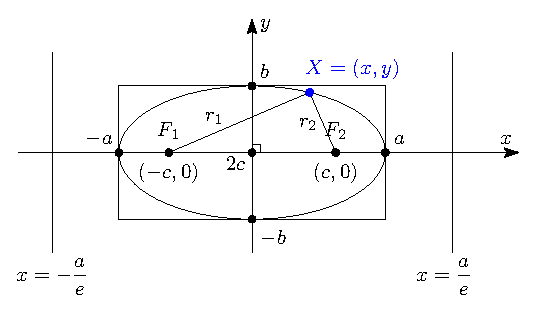
\includegraphics[width=0.5\textwidth]{ANGL3_1.eps}
	\caption{Эллипс в ортогональной СК.}
	\label{3_1}
\end{figure}
Если $a = b$, то у нас будет просто окружность. Пусть у нас есть точка $X = (x,y)$ на этом эллипсе. В прошлый раз мы установили справедливость формул:
$$
	r_1 = |F_1X| = a + \dfrac{c}{a}x, \, r_2 = |F_2X| = a - \dfrac{c}{a}x
$$
\begin{defn}
	\uwave{Эксцентриситетом эллипса} называется следующая величина: $e = \dfrac{c}{a}$.
\end{defn}
\begin{rem}
	Для окружности будет верно: $e = 0$, а также заметим, что у эллипса $e <1$ всегда.
\end{rem}
\begin{defn}
	\uwave{Директриссами эллипса} называется следующее множество точек: $x = \pm \dfrac{a}{e}$.
\end{defn}
\begin{rem}
	Поскольку $e < 1$, то будет верно, что $|x| > a$. Также заметим, что у окружности директрисс нет, поскольку $e = 0$.
\end{rem}

\begin{defn}
	\uwave{Фокальным параметром эллипса} называется следующая величина: $p = \dfrac{b^2}{a}$.
\end{defn}

\subsection*{Гипербола}
\begin{defn}
	\uwave{Гипербола} - это множество точек, координаты которых в некоторой ортогональной декартовой системе координат удовлетворяют уравнению:
	$$
		\dfrac{x^2}{a^2} - \dfrac{y^2}{b^2} = 1, \, a,b > 0
	$$
\end{defn}
\begin{rem}
	Заметим следующее:
	$$
		\dfrac{x^2}{a^2} = 1 + \dfrac{y^2}{b^2} \geq 1 \Rightarrow x^2 \geq a^2 \Rightarrow |x| > a
	$$
	Следовательно, кривая будет лежать вне основного прямоугольника.
\end{rem}

\begin{figure}[H]
	\centering
	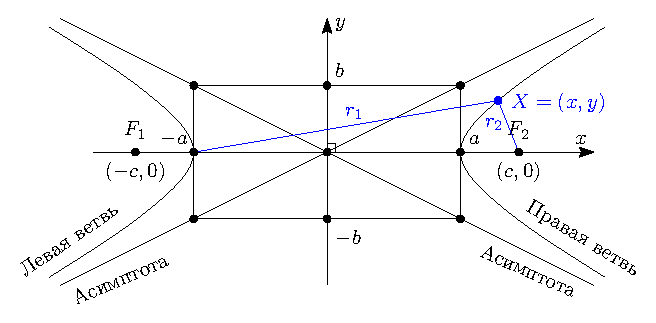
\includegraphics[width=0.6\textwidth]{ANGL3_2.eps}
	\caption{Гипербола в ортогональной СК.}
	\label{3_2}
\end{figure}

\begin{defn}
	\uwave{Асимптотой гиперболы} называются следующие прямые: $y = \pm \dfrac{b}{a}x$.
\end{defn}
\begin{defn}
	\uwave{Фокусами гиперболы} называются точки: $F_1 = (-c,0), \, F_2 = (c,0)$, где $c = \sqrt{a^2 + b^2}$.
\end{defn}
\begin{prop}
	Алгебраическое и геометрическое определения гиперболы эквивалентны.
\end{prop}
\begin{proof}\hfill
	
	$(\Rightarrow)$ Возьмем некоторую точку $X = (x,y)$ на гиперболе. Расстояния от неё до $F_1, \, F_2$ равно $r_1, \, r_2$ соответственно. Найдем $r_1$ по аналогии с эллипсом:
	$$
		r_1 = \sqrt{(x + c)^2 + y^2} = \sqrt{(x+c)^2 +  \dfrac{b^2}{a^2}x^2 - b^2} = \sqrt{x^2 + 2xc + c^2 +  \dfrac{b^2}{a^2}x^2 - b^2 } = 
	$$
	$$
		=\sqrt{\dfrac{c^2}{a^2}x^2 + 2xc + a^2} = \sqrt{\left(a + \dfrac{c}{a}x\right)^2} = \left|a + \dfrac{c}{a}x \right| = 
		\begin{cases}
			a + \dfrac{c}{a}x, & \text{Правая ветвь}\\[8pt]
			-a-\dfrac{c}{a}x, & \text{Левая ветвь}
		\end{cases}
	$$
	Аналогично:
	$$
		r_2 = \left| a - \dfrac{c}{a}x\right| = 
		\begin{cases}
			- a + \dfrac{c}{a}x, & \text{Правая ветвь}\\[8pt]
			a-\dfrac{c}{a}x, & \text{Левая ветвь}
		\end{cases}
	$$
	Рассмотрим правую ветвь:
	$$
		|r_1 - r_2| = |2a| = 2a
	$$
	Аналогично для левой ветви:
	$$
		|r_1 - r_2| = |-2a| = 2a
	$$
	То есть, если $X = (x,y)$ удовлетворяет аналитическому уравнению гиперболы, то это точка гиперболы с фокусами $F_1, \, F_2$ и $||XF_1| - |XF_2|| = 2a$.
	
	$(\Leftarrow)$ Пусть у нас есть ГМТ, таких, что $||XF_1| - |XF_2|| = 2a$ и $|F_1F_2| = 2c$. Как и ранее выбираем центр в качестве начала координат, выбираем оси $x$ и $y$, как и ранее. Тогда возникает условие:
	$$
		\left|\sqrt{(x + c)^2 + y^2 } - \sqrt{(x-c)^2 + y^2}\right| = 2a
	$$
	\begin{exrc}
		Доказать по аналогии с эллипсом и довести до аналитического уравнения, но при этом необходимо рассмотреть два случая.
	\end{exrc}
	Рассмотрим два случая:
	\begin{enumerate}[label=\arabic*)]
		\item $\sqrt{(x + c)^2 + y^2 } - \sqrt{(x-c)^2 + y^2} = 2a$, тогда:
		$$
			(x + c)^2 + y^2 = 4a^2 + (x-c)^2 + y^2 + 4a\sqrt{(x-c)^2 + y^2} \Rightarrow 
		$$
		$$	
			\Rightarrow x^2 + 2xc + c^2 = 4a^2 + x^2 - 2xc + c^2 + 4a\sqrt{(x-c)^2 + y^2} \Rightarrow
		$$
		$$
			\Rightarrow xc - a^2 = a\sqrt{(x-c)^2 + y^2} \Rightarrow x^2c^2 - 2xca^2 + a^4 = a^2{\cdot}\left(x^2 - 2xc + c^2 + y^2\right) \Rightarrow
		$$
		$$
			\Rightarrow x^2(c^2 - a^2)  -a^2y^2 = a^2c^2 - a^4 \Rightarrow x^2(c^2 - a^2) - a^2y^2 = a^2{\cdot}(c^2 - a^2) = a^2b^2 \Rightarrow \dfrac{x^2}{a^2}- \dfrac{y^2}{c^2 - a^2} = 1
		$$
		\item $\sqrt{(x-c)^2 + y^2} - \sqrt{(x + c)^2 + y^2 } = 2a$, тогда:
		$$
			x^2 - 2xc + c^2 + y^2 = 4a^2 + x^2 + 2xc + c^2 + 4a\sqrt{(x + c)^2 + y^2 } \Rightarrow 
		$$
		$$
			\Rightarrow -xc - a^2 = a{\cdot}\sqrt{(x + c)^2 + y^2} \Rightarrow x^2c^2 + 2xca^2 + a^4 = a^2{\cdot}\left(x^2 + 2xc + c^2 + y^2\right)  \Rightarrow
		$$
		$$
			\Rightarrow x^2(c^2 - a^2) -a^2y^2 = a^2{\cdot}(c^2 - a^2) \Rightarrow \dfrac{x^2}{a^2} - \dfrac{y^2}{c^2 - a^2} = 1
		$$
	\end{enumerate}
	Таким образом, в обоих случаях мы получаем аналитическое уравнение для: 
	$$
		b = \sqrt{c^2 - a^2}
	$$
	По аналогии с эллипсом $c > a \Rightarrow b >0$. При этом никаких конкретных отношений между $a$ и $b$ здесь установить нельзя.
\end{proof}

\begin{defn}
	\uwave{Эксцентриситетом гиперболы} называется следующая величина: $e = \dfrac{c}{a}$.
\end{defn}
\begin{rem}
	Заметим, что:
	$$
		c = \sqrt{a^2 + b^2}, \, b \neq 0 \Rightarrow c > a \Rightarrow e > 1
	$$
	то есть эксцентриситет гиперболы всегда больше $1$.
\end{rem}
\begin{defn}
	\uwave{Директриссами гиперболы} называется следующее множество точек: $x = \pm \dfrac{a}{e}$.
\end{defn}

\begin{rem}
	Поскольку $|e| > 1$, то будет верно, что $|x| < a$ для директрисс.
\end{rem}

\begin{figure}[H]
	\centering
	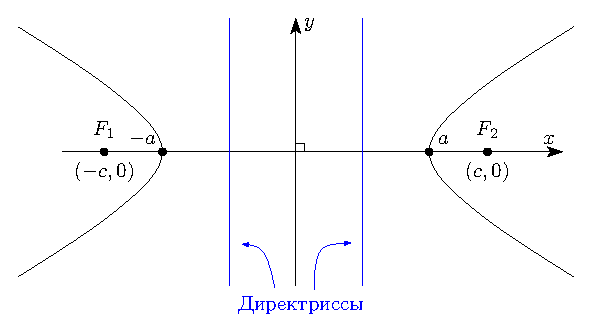
\includegraphics[width=0.5\textwidth]{ANGL3_3.eps}
	\caption{Директриссы гиперболы.}
	\label{3_3}
\end{figure}

\begin{defn}
	\uwave{Фокальным параметром гиперболы} называется следующая величина: $p = \dfrac{b^2}{a}$.
\end{defn}

\begin{figure}[H]
	\centering
	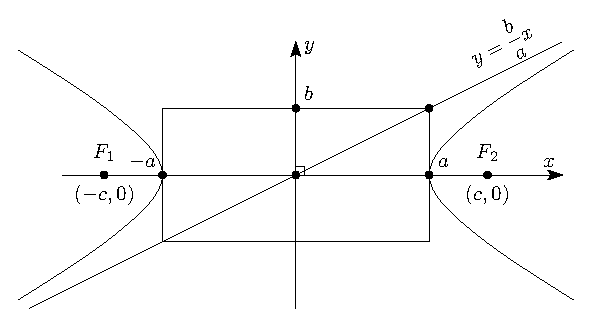
\includegraphics[width=0.6\textwidth]{ANGL3_4.eps}
	\caption{Асимптота гиперболы.}
	\label{3_4}
\end{figure}

\begin{prop}
	При $|x| \to \infty$, гипербола стремится к своим асимптотам, не пересекая их.
\end{prop}
\begin{proof}
	Заметим, что в каждом квадранте системы координат у нас есть своя ветвь гиперболы и асимптота. Рассмотрим первый квадрант, тогда:
	$$
		y_{as} = \dfrac{b}{a}x, \, y = \sqrt{\dfrac{b^2}{a^2}x^2 - b^2} \Rightarrow \Delta(x) = y_{as}(x) - y(x) = 	\dfrac{b}{a}x -  \sqrt{\dfrac{b^2}{a^2}x^2 - b^2} = \dfrac{b}{a}\left(x - \sqrt{x^2 - a^2}\right) = 
	$$
	$$
		= \dfrac{b}{a}{\cdot}\dfrac{a^2}{x + \sqrt{x^2 - a^2}} \xrightarrow[x \to \infty]{} 0, \, |x| \geq a \Rightarrow \forall x > 0, \, \Delta(x) > 0
	$$
	Если бы хоть где-то была точка пересечения, то где-то было бы верно, что $\Delta(x) = 0$. Следовательно, гипербола стремится к своей асимптоте, не пересекая её. Аналогичное будет верно и для других квадрантов.
\end{proof}

\newpage
\subsection*{Парабола}

\begin{defn}
	\uwave{Параболой} называется ГМТ, равноудаленных от фокуса параболы и директриссы параболы. 
\end{defn}

\begin{defn}
	\uwave{Параболой} называется множество точек, координаты которых в подходящей системе координат удовлетворяют следующему уравнению:
	$$
		y^2 = 2px, \, p > 0
	$$
\end{defn}

\begin{prop}
	Алгебраическое и геометрическое определения параболы эквивалентны.
\end{prop}
\begin{proof}\hfill\\
	$(\Leftarrow)$ Пусть у нас задан фокус $F$, задана директрисса $d$ и мы рассматриваем ГМТ таких, что расстояния от этих точек до директриссы - равны. Введем координаты следующим образом: ось $x$ расположим по оси параболы (прямая, проходящая через фокус параболы оротогонально директриссе), ось $y$ расположим посередине между директриссой и параболой (поскольку там расстояние от директриссы до параболы будет равно расстоянию от параболы до фокуса), ортогонально оси $x$.
	
	\begin{figure}[H]
		\centering
		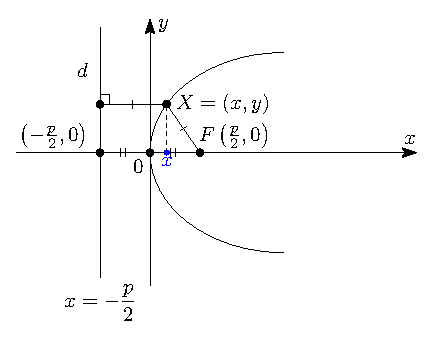
\includegraphics[width=0.45\textwidth]{ANGL3_5.eps}
		\caption{Геометрическое определение параболы.}
		\label{3_5}
	\end{figure}
	Пусть координаты фокуса равны $F = \left(\tfrac{p}{2},0\right)$, рассмотрим точку $X = (x,y)$ на парабооле, тогда:
	$$
		|XF| = \sqrt{\left(x - \dfrac{p}{2}\right)^2 + y^2}, \, \rho(X,d) = x + \dfrac{p}{2} \Rightarrow \left(x - \dfrac{p}{2}\right)^2 + y^2 = \left(x + \dfrac{p}{2}\right)^2 \Rightarrow
	$$
	$$
		\Rightarrow x^2 - px + \dfrac{p^2}{4} + y^2 = x^2 + px + \dfrac{p^2}{4} \Rightarrow y^2 = 2px
	$$
	
	$(\Rightarrow)$ Пусть наши точки удовлетворяют уравненияю: $y^2 = 2px, \, p > 0$. Очевидно, что это перевернутая парабола (известная со школы), её минимум будет в точке $0$. Рассмотрим некоторую точку $X(x,y)$ на параболе, затем возьмем прямую $x = -\tfrac{p}{2}$ и фокус с координатами $F\left(\tfrac{p}{2}, 0\right)$, тогда:
	$$
		|XF| = \sqrt{\left(x - \dfrac{p}{2}\right)^2 + y^2} = \sqrt{\left(x - \dfrac{p}{2}\right)^2 + 2px} = \sqrt{\left(x + \dfrac{p}{2}\right)^2} = \left| x + \dfrac{p}{2}\right| = x + \dfrac{p}{2} = \rho(X,d) 
	$$
	\begin{figure}[H]
		\centering
		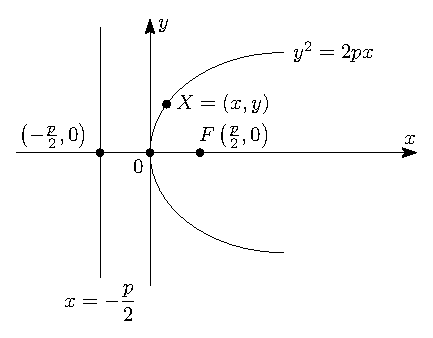
\includegraphics[width=0.45\textwidth]{ANGL3_6.eps}
		\caption{Аналитическое определение параболы.}
		\label{3_6}
	\end{figure}
	Таким образом, если мы используем заданное аналитическое уравнение, то автоматически имеем геометрическое свойство.
\end{proof}

\begin{defn}
	\uwave{Фокусом параболы} называется точка: $F = \left(\tfrac{p}{2},0\right)$.
\end{defn}

\begin{defn}
	\uwave{Директриссой параболы} называется прямая: $x = -\dfrac{p}{2}$.
\end{defn}

\begin{defn}
	\uwave{Фокальным параметром параболы} называется величина: $p$.
\end{defn}

\begin{defn}
	\uwave{Эксцентриситетом параболы} называется величина: $e = 1$.
\end{defn}

\newpage
\section*{Характеристические числа коник}

\subsection*{Фокальный параметр}
В каждой из наших коник, проведём хорду из фокуса, перпендикулярно оси $y$.

\begin{defn}
	\uwave{Фокальной хордой} называется перпендикуляр, проведённый из фокуса коники к самой конике.
\end{defn}
\begin{figure}[H]
	\centering
	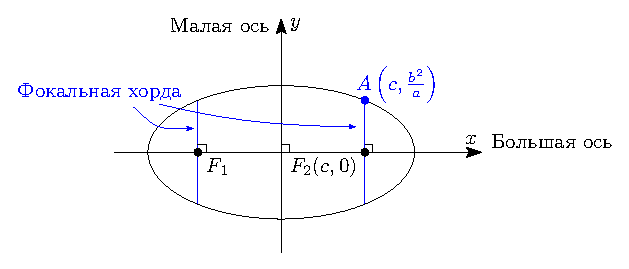
\includegraphics[width=0.6\textwidth]{ANGL3_7.eps}
	\caption{Фокальная хорда эллипса.}
	\label{3_7}
\end{figure}
\begin{figure}[H]
	\centering
	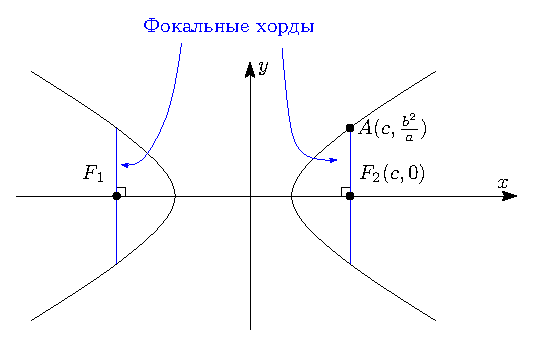
\includegraphics[width=0.45\textwidth]{ANGL3_8.eps}
	\caption{Фокальная хорда гиперболы.}
	\label{3_8}
\end{figure}
\begin{figure}[H]
	\centering
	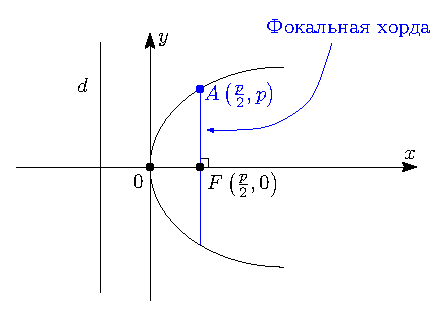
\includegraphics[width=0.45\textwidth]{ANGL3_9.eps}
	\caption{Фокальная хорда параболы.}
	\label{3_9}
\end{figure}

\begin{prop}
	Длина любой фокальной хорды равна удвоенному фокальному параметру $p$, для любой коники.
\end{prop}
\begin{proof}\hfill
	\begin{enumerate}[label=\arabic*)]
		\item \textbf{Парабола}: воспользуемся аналитической формулой коники:
		$$
			F = \left(\dfrac{p}{2}, 0\right) \Rightarrow y^2 = 2p{\cdot}\dfrac{p}{2} = p^2 \Rightarrow A = \left(\dfrac{p}{2},p\right) \Rightarrow |AF| = p
		$$
		\item \textbf{Эллипс}: возьмем точку $F_2$ и воспользуемся аналитической формулой коники:
		$$
			\dfrac{c^2}{a^2} + \dfrac{y^2}{b^2} = 1 \Rightarrow y^2 = b^2 - \dfrac{b^2c^2}{a^2} = b^2{\cdot}\left(\dfrac{a^2 - c^2}{a^2}\right) = \dfrac{b^4}{a^2} \Rightarrow 
		$$
		$$	
			\Rightarrow y = \dfrac{b^2}{a} \Rightarrow A = \left(c, \dfrac{b^2}{a}\right) \Rightarrow |AF| = \dfrac{b^2}{a} = p
		$$
		\item \textbf{Гипербола}: возьмем точку $F_2$ и воспользуемся аналитической формулой коники:
		$$
			\dfrac{c^2}{a^2} - \dfrac{y^2}{b^2} = 1 \Rightarrow y^2 = \dfrac{b^2c^2}{a^2} - b^2 = b^2{\cdot}\left(\dfrac{c^2 - a^2}{a^2}\right) = \dfrac{b^4}{a^2} \Rightarrow 
		$$
		$$	
			\Rightarrow y = \dfrac{b^2}{a} \Rightarrow A = \left(c, \dfrac{b^2}{a}\right) \Rightarrow |AF_2| = \dfrac{b^2}{a} = p
		$$
	\end{enumerate}
\end{proof}

\subsection*{Директориальное свойство коник}

\begin{prop}(\textbf{директориальное свойство коник})
	Отношение расстояний от точки коники до фокуса и до соответствующей директриссы равно эксцентриситету.	
\end{prop}


\begin{proof}\hfill
	\begin{enumerate}[label=\arabic*)]
		\item \textbf{Парабола}: мы знаем, что в параболе расстояние от любой точки на ней до директриссы и до фокуса - равны, запишем это в следующем виде:
		$$
			\forall X = (x,y) \colon y^2 = 2px \Rightarrow \rho(X,F) = \rho(X,d) \Rightarrow \dfrac{\rho(X,F)}{\rho(X,d)} = e = 1
		$$
		\begin{figure}[H]
			\centering
			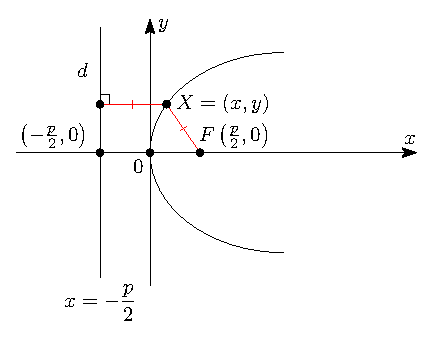
\includegraphics[width=0.35\textwidth]{ANGL3_10.eps}
			\caption{Расстояния от параболы до фокуса и директриссы - равны.}
			\label{3_10}
		\end{figure}
		\item \textbf{Эллипс}: посчитаем расстояние от точки до фокуса и от точки до директриссы, которая находится на той же стороне, что и фокус:
		$$
			\forall X = (x,y) \colon \dfrac{x^2}{a^2} + \dfrac{y^2}{b^2} = 1 \Rightarrow \rho(X,F_1) = r_1 = a + \dfrac{c}{a}x = a + ex
		$$
		\begin{figure}[H]
			\centering
			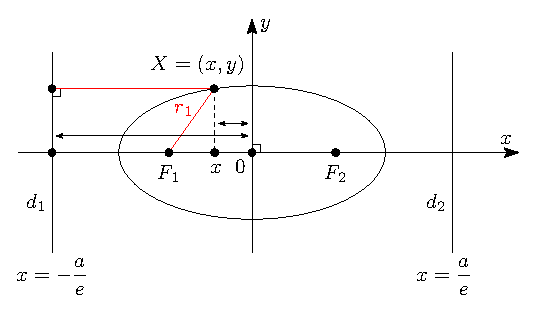
\includegraphics[width=0.45\textwidth]{ANGL3_11.eps}
			\caption{Расстояния от эллипса до фокуса и директриссы.}
			\label{3_11}
		\end{figure}
		$$
			\rho(X,d_1) = x - \left(-\dfrac{a}{e}\right) = x + \dfrac{a}{e} \Rightarrow \dfrac{\rho(X,F)}{\rho(X,d)} = \dfrac{a + ex}{a + ex}{\cdot}e = e
		$$
		\item \textbf{Гипербола}: по аналогии с эллипсом:
		$$
			\forall X = (x,y)\colon \dfrac{x^2}{a^2} - \dfrac{y^2}{b^2} = 1 \Rightarrow \rho(X,F_1) = r_1 = \left| a + \dfrac{c}{a}x\right|  = |a + ex|
		$$
		Для левой ветви:
		$$
			\rho(X,d_1) = \left(-\dfrac{a}{e}\right) - x = -\dfrac{a + ex}{e}
		$$
		Для правой ветви:
		$$
			\rho(X,d_1) = x - \left(-\dfrac{a}{e}\right) = \dfrac{a + ex}{e}
		$$
		Тогда:
		$$
			\rho(X,d_1) = \left|\dfrac{a + ex}{e} \right| \Rightarrow \dfrac{\rho(X,F)}{\rho(X,d)} = \dfrac{|a + ex|}{|a + ex|}{\cdot}|e| = |e| = e
		$$
	\end{enumerate}
\end{proof}

\begin{rem}
	Заметим, что наше геометрическое определение параболы это в точности директориальное свойство параболы. На самом деле, мы можем так определить любую конику (и эллипс, и параболу): выбираем фокус $F$ (некоторая точка), выбираем директриссу $d$ (некоторая прямая), выбираем $e$ и рассматриваем ГМТ, определенных соотношением:
	$$
		e = \dfrac{\rho(X,F)}{\rho(X,d)}
	$$
\end{rem}

\begin{exrc}
	Доказать, что такое определение эквивалентно определению коник.
\end{exrc}

\section*{Полярные координаты}

Из школы известно, что декартова система координат задается выбором начала системы координат и двух ортогональных осей, которые через неё проходят. Полярная система координат задается точкой и лучом, который из неё выходит.
\begin{defn}
	\uwave{Полюсом} называется нулевая точка в полярной системе координат.
\end{defn}
\begin{defn}
	\uwave{Полярной осью} называется ось в полярной системе координат.
\end{defn}

Чтобы охарактеризовать точку в такой системе координат, проводится отрезок соединяющий полюс и эту точку. У этого отрезка есть длина: $r = |OA| \geq 0$, в качестве второй координаты выбирается угол $\varphi$, который отчитывается от полярной оси против часовой стрелки.

\begin{figure}[H]
	\centering
	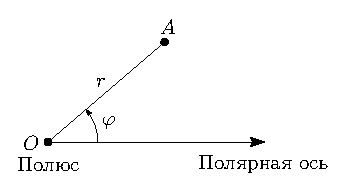
\includegraphics[width=0.3\textwidth]{ANGL3_12.eps}
	\caption{Полярная система координат.}
	\label{3_12}
\end{figure}

Тогда имея $r$ и $\varphi$, мы всегда сможем однозначно построить точку: $A = (r,\varphi)$.
\begin{rem}
	Тем не менее по точке координаты определяются не всегда однозначно, поскольку у полюса не определена координата $\varphi$.
\end{rem}
\begin{rem}
	Кроме того, угол можно определить с точностью до $2\pi$.
\end{rem}
\begin{rem}
	Также заметим, что всегда верно: $r \geq 0$.
\end{rem}

Полярные координаты удобны тем, что в них некоторые объекты хорошо описываются, например те, которые имеют круговую симметрию. Уравнение окружности у которой радиус равен $2$, а центр в полюсе будет иметь вид: 
$$
	r = 2
$$

У нас возникает задача по выбору того, куда мы поставим полюс и полярную ось в конике.
\begin{enumerate}[label=\arabic*)]
	\item \textbf{Эллипс}: расположим полюс в фокусе $F_1$, а полярную ось проведём через второй фокус:
	\begin{figure}[H]
		\centering
		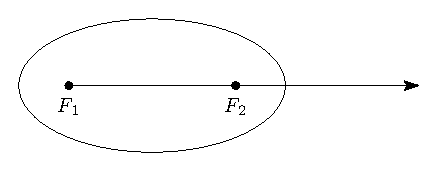
\includegraphics[width=0.35\textwidth]{ANGL3_13.eps}
		\caption{Полярная система координат: эллипс.}
		\label{3_13}
	\end{figure}
	\item \textbf{Гипербола}: расположим полюс в одном из фокусов ($F_2$), а полярную ось провёдем в сторону, противоположную другому фокусу:
	\begin{figure}[H]
		\centering
		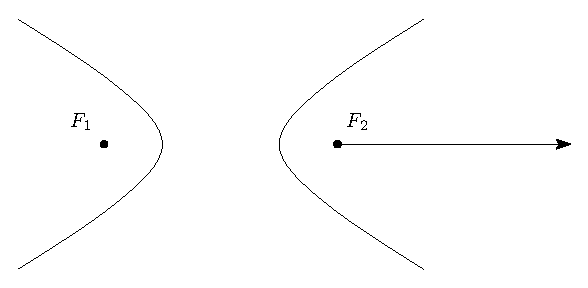
\includegraphics[width=0.45\textwidth]{ANGL3_14.eps}
		\caption{Полярная система координат: гипербола.}
		\label{3_14}
	\end{figure}
	\item \textbf{Парабола}: расположим полюс в фокусе $F$, а полярную ось провёдем вдоль оси параболы от директриссы в сторону:
	\begin{figure}[H]
		\centering
		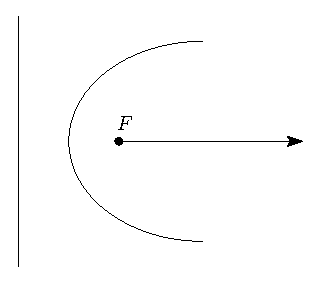
\includegraphics[width=0.25\textwidth]{ANGL3_15.eps}
		\caption{Полярная система координат: парабола.}
		\label{3_15}
	\end{figure}
\end{enumerate}

\begin{prop}
	В полярных координатах, выбранных указанным выше способом, уравнения эллипса, параболы и правой ветви гиперболы будет иметь вид:
	$$
		r = \dfrac{p}{1 - e{\cdot}\cos{(\varphi)}}
	$$
	Уравнение левой ветви гиперболы будет иметь вид:
	$$
		r = -\dfrac{p}{1 + e{\cdot}\cos{(\varphi)}}
	$$
\end{prop}
\begin{proof}
	Воспользуемся директориальным свойством коник:
	\begin{enumerate}[label=\arabic*)]
		\item \textbf{Эллипс}: возьмем точку $X(r,\varphi)$ на эллипсе, тогда:
		$$
			|XF_1| = r, \, \rho(F_1,d) =\dfrac{a}{e} - c 
		$$
		Чтобы найти расстояние от $X$ до директриссы построим перпендикуляр из полюса к прямой от $X$ к директриссе, тогда:
		$$
			\rho(F_1,d) = \dfrac{a}{e} - c, \, \rho(A,X) = r{\cdot}\cos{(\varphi)} \Rightarrow \rho(X,d) = \dfrac{a}{e} - c + r{\cdot}\cos{(\varphi)}
		$$
		\begin{figure}[H]
			\centering
			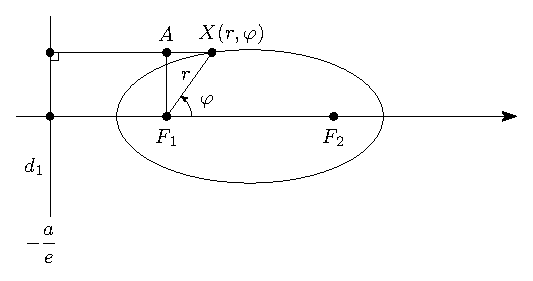
\includegraphics[width=0.5\textwidth]{ANGL3_16.eps}
			\caption{Уравнение эллипса в полярных координатах.}
			\label{3_16}
		\end{figure}
		Тогда:
		$$
			\dfrac{|XF_1|}{\rho(X,d)} = e \Leftrightarrow \dfrac{r}{\dfrac{a}{e} - c + r{\cdot}\cos{(\varphi)}} = e \Leftrightarrow r = a - ec + er{\cdot}\cos{(\varphi)} \Rightarrow r = \dfrac{a - ec}{1 - e{\cdot}\cos{(\varphi)}}
		$$
		$$
			a - ec = a - \dfrac{c}{a}{\cdot}c = \dfrac{a^2 - c^2}{a} = \dfrac{b^2}{a} = p \Rightarrow  r = \dfrac{p}{1 - e{\cdot}\cos{(\varphi)}}
		$$
		\item \textbf{Парабола}: аналогично, возьмем точку $X(r,\varphi)$ на параболе, тогда:
		$$
			|XF| = r = \rho(X,d), \, \rho(F,d) = \dfrac{p}{2} - \left(-\dfrac{p}{2}\right) = p
		$$
		$$
			r = \rho(X,d) = \rho(F,d) + r{\cdot}\cos{(\varphi)} = p + r{\cdot}\cos{(\varphi)}
		$$
		$$
			\dfrac{|XF|}{\rho(X,d)} = e = 1 \Leftrightarrow \dfrac{r}{p + r{\cdot}\cos{(\varphi)}} = 1 \Leftrightarrow r = \dfrac{p}{1- \cos{(\varphi)}} = \dfrac{p}{1 - e{\cdot}\cos{(\varphi)}}
		$$
		\item \textbf{Обе ветви гиперболы}: аналогично, в том числе одна из ветвей доказывается через центральную симметричность;
	\end{enumerate}
\end{proof}

\begin{exrc}
	(**) Вывести директориальное свойство, используя шары Данделена.
\end{exrc}
\begin{rem}
	Данное доказательство крайне сложное и должно убедить нас, что аналитический подход гораздо лучше.
\end{rem}

\end{document}